\documentclass[uplatex]{jsarticle}
\usepackage{listings}
\lstset{
  basicstyle={\ttfamily},
  identifierstyle={\small},
  commentstyle={\smallitshape},
  keywordstyle={\small\bfseries},
  ndkeywordstyle={\small},
  stringstyle={\small\ttfamily},
  frame={tb},
  breaklines=true,
  columns=[l]{fullflexible},
  numbers=left,
  xrightmargin=0zw,
  xleftmargin=3zw,
  numberstyle={\scriptsize},
  stepnumber=1,
  numbersep=1zw,
  lineskip=-0.5ex
}
\usepackage[dvipdfmx]{graphicx}
\title{画像認識 レポート1}

\author{101730153 佐治 礼仁 saji.ayahito@h.mbox.nagoya-u.ac.jp}
\date{\today}
\begin{document}
\maketitle
\section{画像上への任意の文字列の重畳表示}
Colabで実装した.ソースコードをListing \ref{list:source}に示す.
\begin{lstlisting}[caption=画像への文字列の重畳処理,label=list:source]
import numpy as np
import cv2
import matplotlib.pyplot as plt

from google.colab import files
from google.colab.patches import cv2_imshow

from google.colab import drive

drive.mount('/content/drive/')
%cd "/content/drive/My Drive/Colab Notebooks/"

img=cv2.imread('./images/nagoya.jpg')
if img is None:
    print('file not found.')

cv2.putText(img, 'Nagoya', (40,480), cv2.FONT_HERSHEY_SCRIPT_SIMPLEX,3,(255,255,255),4)
cv2_imshow(img)
\end{lstlisting}
\section{結果}
結果として出力された画像を図\ref{fig:result}に示す.正しく画像中に文字列が表示されていることが確かめられた.
\begin{figure}[htbp]
  \begin{center}
    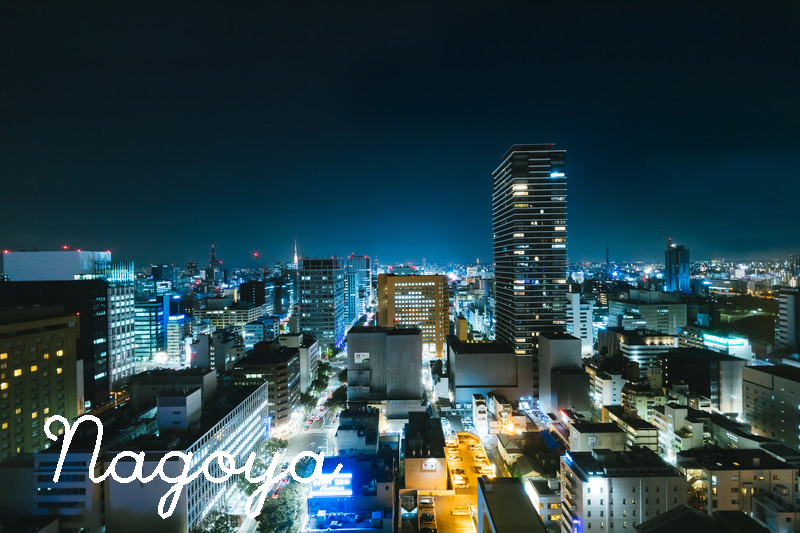
\includegraphics[clip,width=10.0cm]{figures/image2.png}
    \caption{出力されたnagoyaという文字列が重畳された画像}
    \label{fig:result}
  \end{center}
\end{figure}

\end{document}
